%!TEX root =  A_WS.tex

\section*{Practice Exam 3B}  
\markright{Practice Exam 3B}  
\addcontentsline{toc}{section}{Practice Exam 3B}

\emph{Try taking this version of the practice exam under testing conditions:  no book, no notes, no classmate's help, no electronics (computer, cell phone, television). Give yourself one hour to work and wait until you have tried your best on all of the problems before checking any answers.} \bigskip

\noindent \textbf{Caution:} Usually more than half points on this exam are for solving equations and inequalities. Be sure you understand what you need to show for full credit.  Using a different method, or not showing enough work might get little to no partial credit. \bigskip

\noindent \hrulefill

\begin{enumerate}

\item Goldie the Goldfish, Pinches the Lobster, Quackers the Duck, Speedy the Turtle.  These first generation Beanie Babies toys were anticipated to increase in value according to the equation $$B = 6\ast1.08^Y$$ where $B$ is the value of Beanie Babies (in \$) and Y is the years since 1994. 

\hfill \begin{footnotesize} These names are registered trademarked. \end{footnotesize}
\begin{enumerate}
\item Make a table showing the anticipated value in 1994, 2004, 2010, and 2025.  \vfill 
\item Draw a graph showing how the value of the Beanie Babies increased. 
\begin{center}
\scalebox {.8} {
\includegraphics [width = 6in] {GraphPaper.jpg}}
\end{center}
\newpage
\hspace{-.5in}  \emph{The problem continues \ldots}
\item Set up and solve an equation to determine when will Beanie Babies made in 1994 were anticipated to be worth over \$40.  Report the actual year. \vfill 
\end{enumerate} 

\newpage

 \item  Best we can tell, the floor of our front porch was 7'2" above ground when the house was built.  It has been slowly sinking ever since.  The contractor estimated that it's dropped .45 inches per year.  The equation is $$P = 86-.45A$$ where $P$ is the height of the porch (in inches) and $A$ is the age of the house (in years).
\begin{enumerate}
\item Make a table showing the height of the front porch when the house was built, when it was 20 years old, and when it was 50 years old.  \vfill 
\item The floor of our front porch is currently 48 inches above ground.   Set up and solve an equation to figure out how old our house is.  \vfill \vfill 
\item Once the porch is below 40 inches, we will have to do something to fix it. Set up and solve an inequality to find when that will happen, answering to the nearest year.  \emph{Hint:  the house is already old.  Report how many years from now.} \vfill \vfill 
\end{enumerate} 

\newpage

\item In a \textbf{shot put} competition, athletes try to throw a heavy metal ball as far as possible.  For one athlete the ball closely followed the parabolic arch given by the equation $$H = -.015D^{2}+1.04D+5.9 $$ where D was the distance the ball had travelled horizontally and H was the height of the ball above ground, both in feet.  The path of the ball  is graphed below.
\begin{center}
\scalebox {.8} {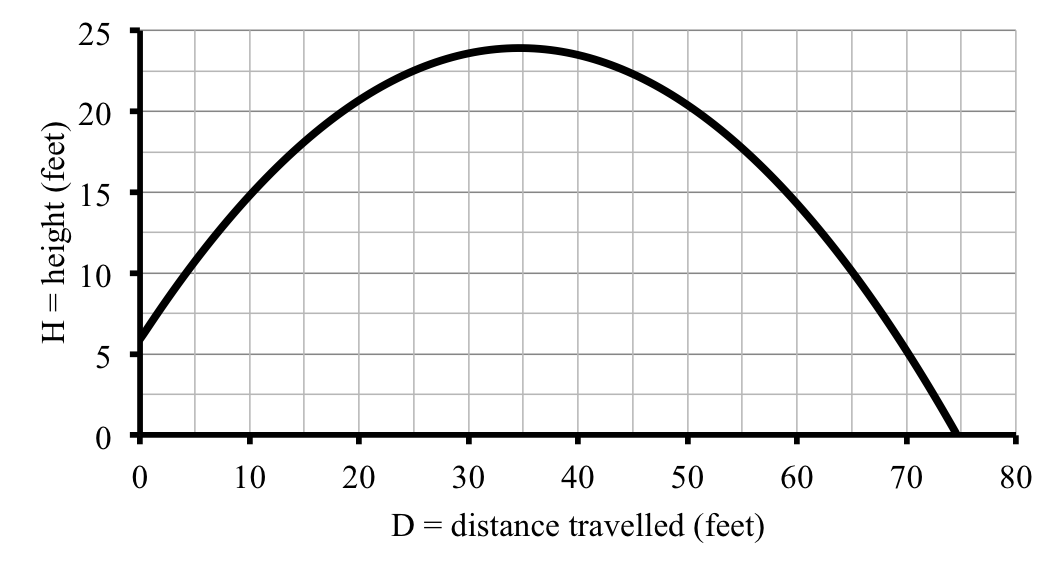
\includegraphics [width = 6in] {shotput.png}}
\end{center}

\begin{enumerate}
\item How far away did the ball land? Estimate the answer from the graph.  Then show how to set up and solve an equation to find the answer to two decimal places. \vfill \vfill \vfill  \vfill
\item How high up did the ball get?  Show how to find the exact answer.  Then compare to the graph.  \vfill 
\end{enumerate}  

\newpage

\item The amount of snow in a snowball, $C$ cups, depends on the \textbf{diameter} (distance across) of the snowball, $D$ inches according to the equation $$C = 0.036D^3$$
\begin{enumerate}
\item How many cups of snow are needed to make a snowball that is 3 inches across? 5 inches across? \vfill 
\item How many cups of snow are needed to make a snowball that is 2 feet across?
Give your answer in gallons.  Use that $1 \text{ gallon} = 4 \text{ quarts}$ and $1 \text{ quart} = 4 \text{ cups}$. \vfill
\item  Karen has a 5 gallon paint bucket packed with snow and wants to make a giant snowball out of it. How big will the snowball be? Show how to use successive approximation to find the answer to the nearest inch. Display your calculations in a table.\vfill \vfill 
\item Now set up and solve an equation to find the answer to the nearest inch. \vfill  \vfill \vfill 
\end{enumerate} 

% END
\end{enumerate}


